\subsection{Using BMS as an oracle to identify S-shaped CV curves}
The application of the BMS oracle to label the CV responses as target, if they are of S-shape, and as non-targets otherwise is demonstrated in this section. 
The proposed BMS oracle is used to label the CV responses and couple it with standard active search techniques to find our "targets" within a given budget of label queries (equivalently number of queries to the simulator). 
To accommodate for the high-throughput search running a batch of experiments at a time, we run the active search using both sequential selection of query locations~(batch size \(b=1\)) and a batch selection~(\(b=100\)). 
We use the  design space in~\Cref{tab:search_space} and aim to find as many targets as possible in the resulting combinatorial design space~\(\mathcal{S}\) of six parameters (dimension of \(\mathcal{S}\)). 

To demonstrate the efficacy of the proposed methods, we first pre-compute labels for a set of ten CV curves in \(\mathcal{S}\) of varying shape.
\Cref{fig:repbmsscores} depicts the chosen CV curves ordered based on model posterior~(\Cref{eq:logPostM}) percentile rank.
Notably, the highest scored CV curves have the S-shape which are of interest in this work.
From~\Cref{fig:repbmsscores}, it can be noted that BMS assigned the highest score to CV curves where the forward and backward sweeps overlap exactly i.e. no hysteresis or capacitive behavior~(highlighted using a red box). 
On the other spectrum, the oracle labels several types of CV curves with low scores.  

The good performance of BMS in this study can be attributed to its inherent ability to handle Gaussian noise, which is also of practical interest for cyclic voltammetry responses~\cite{gavaghan2018use}. 
For comparison, we studied two other oracles to rank a CV curve based on their S-shape characteristics using point-wise comparison: a)~\textit{similarity score} that uses a generic approach of computing the Euclidean norm between a given CV curve and user defined reference S-shape; and b) \textit{FOWA score} that is physics inspired and defined as the \(R^2\)-value for any CV curve in Foot of The Wave Analysis~(FOWA) coordinate space~(a perfect symmetric S-shaped CV curve has \(R^2=1\)). 
% We discuss more details on (a,b) in Supplementary Information. 
\begin{figure}[h]
    \centering
    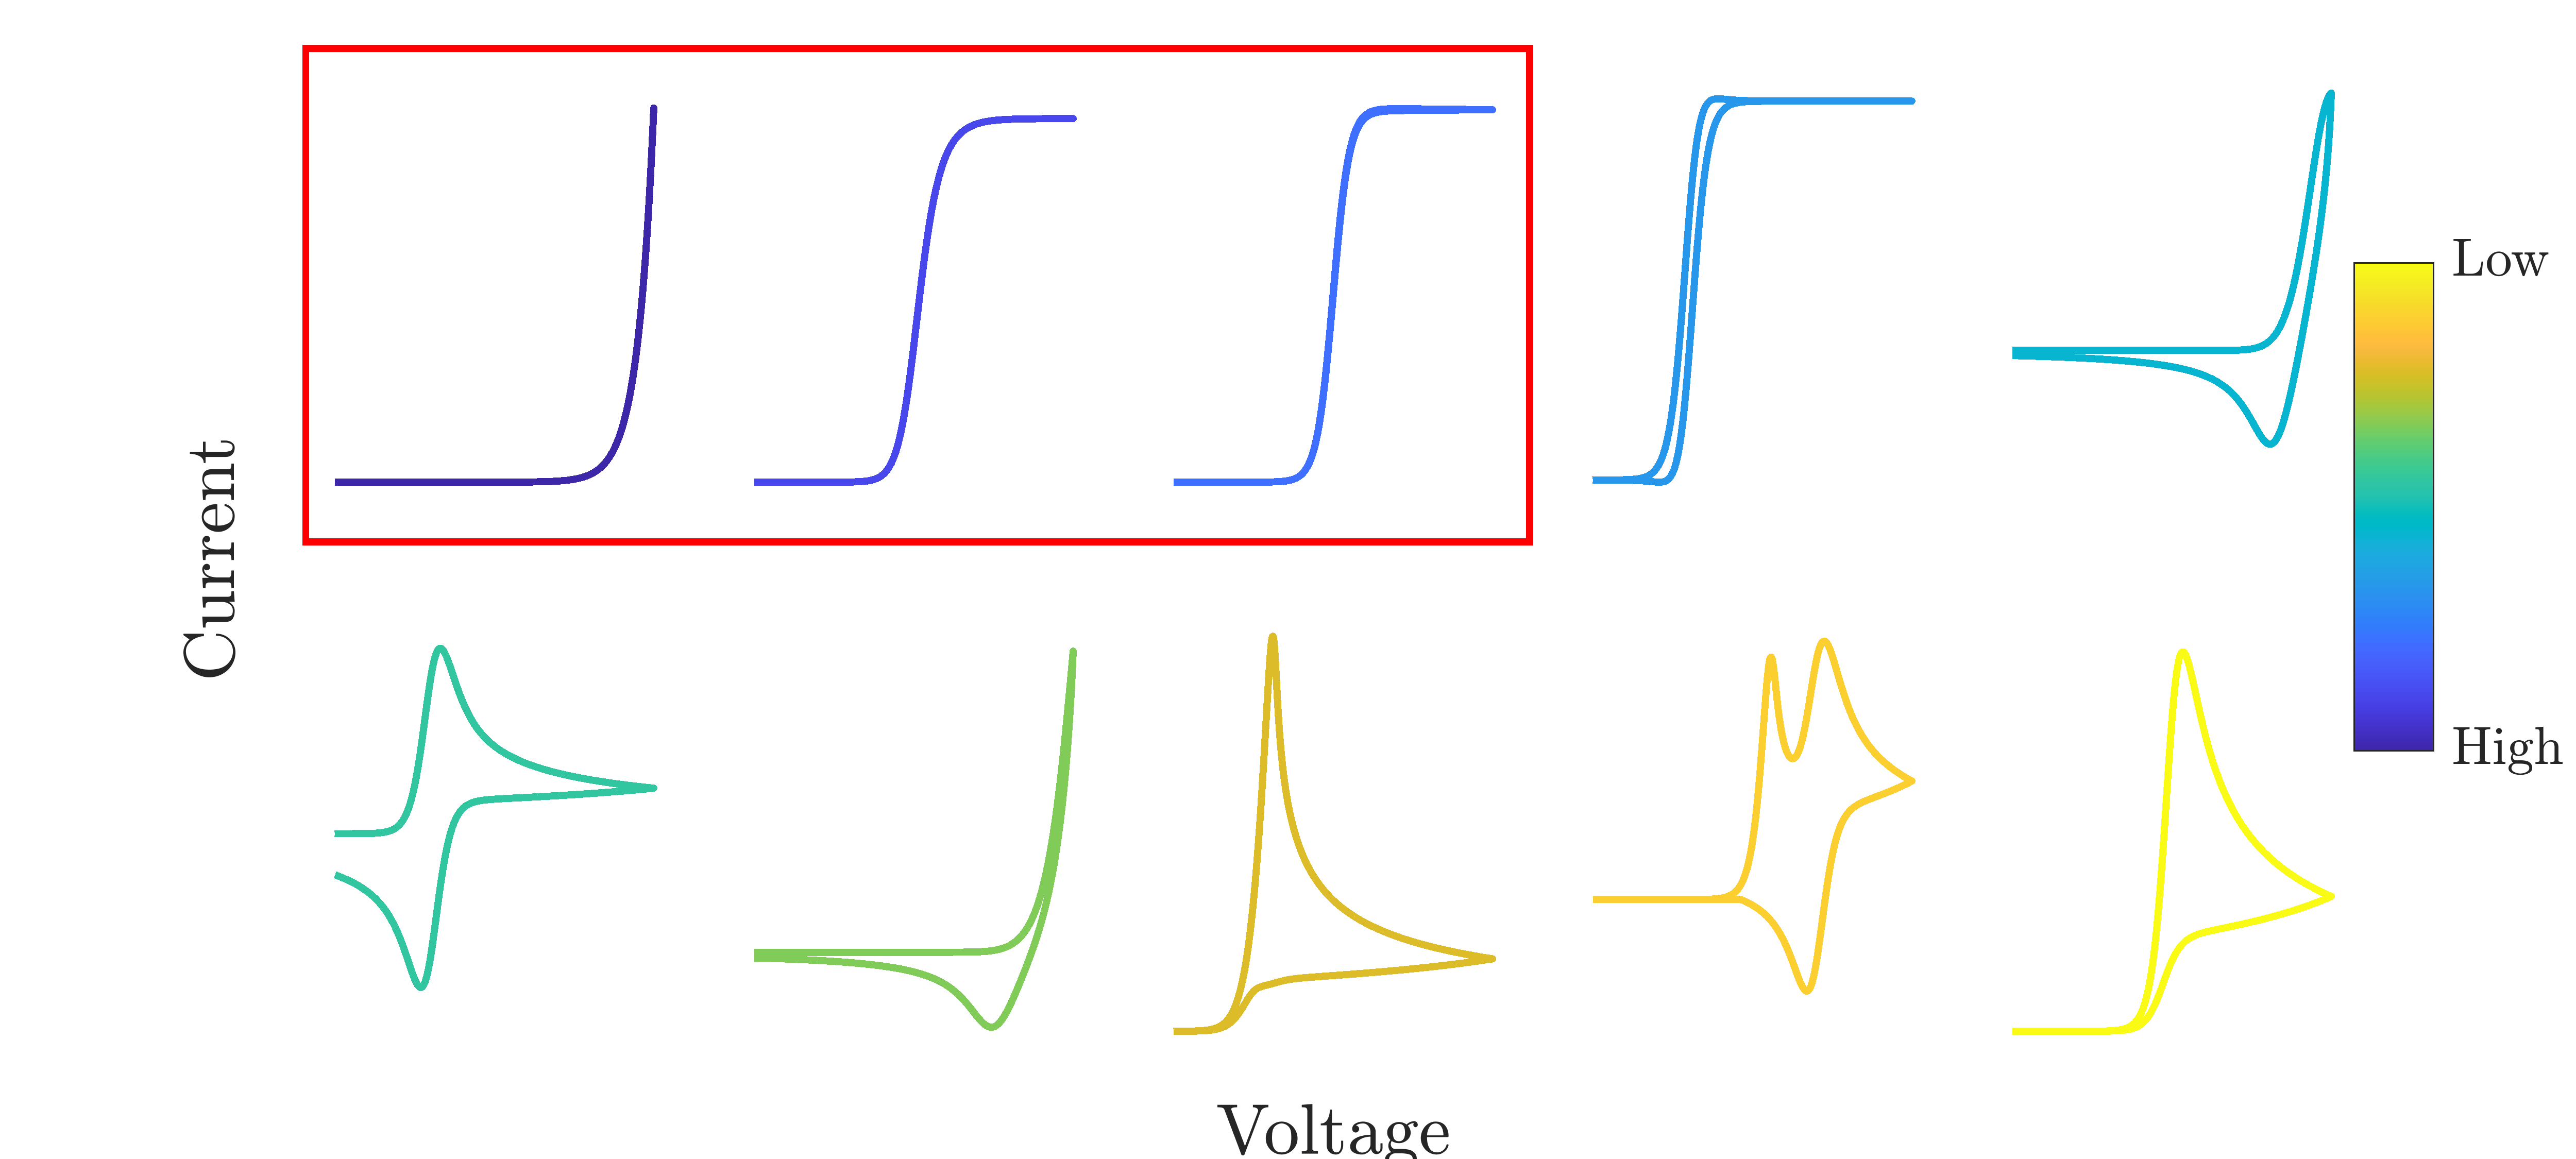
\includegraphics[width=100mm]{Chapter-3/figures/repbmsspectrum.png}
    \caption{Representative CV curves from the dataset ordered and color coded using the BMS score. CV curves boxed in red will be labelled as targets by the oracle.}
    \label{fig:repbmsscores}
\end{figure}

\subsubsection{Similarity score based oracle}
A Euclidean norm between a reference CV curve \(I_{ref}\) and any given CV curve \(I\) is computed using \(\sum \sqrt{(I - I_{ref})^2}\) both represented as vectors in a high-dimensional space and sum taken over the components. 
In~\Cref{figSI:repssscores} ten representative CV curves are depicted by sorting and color-coding based on the similarity score (similar to~\Cref{fig:repbmsscores}). 
The results showcase poor performance of the similarity score and ordering the CV curves with only two targets in the top three.
Although it marks the first curve correctly with high score, it fails to identify other S-shaped curve that is shifted along the voltage with respect to the first curve.
\begin{figure}[h]
    \centering
    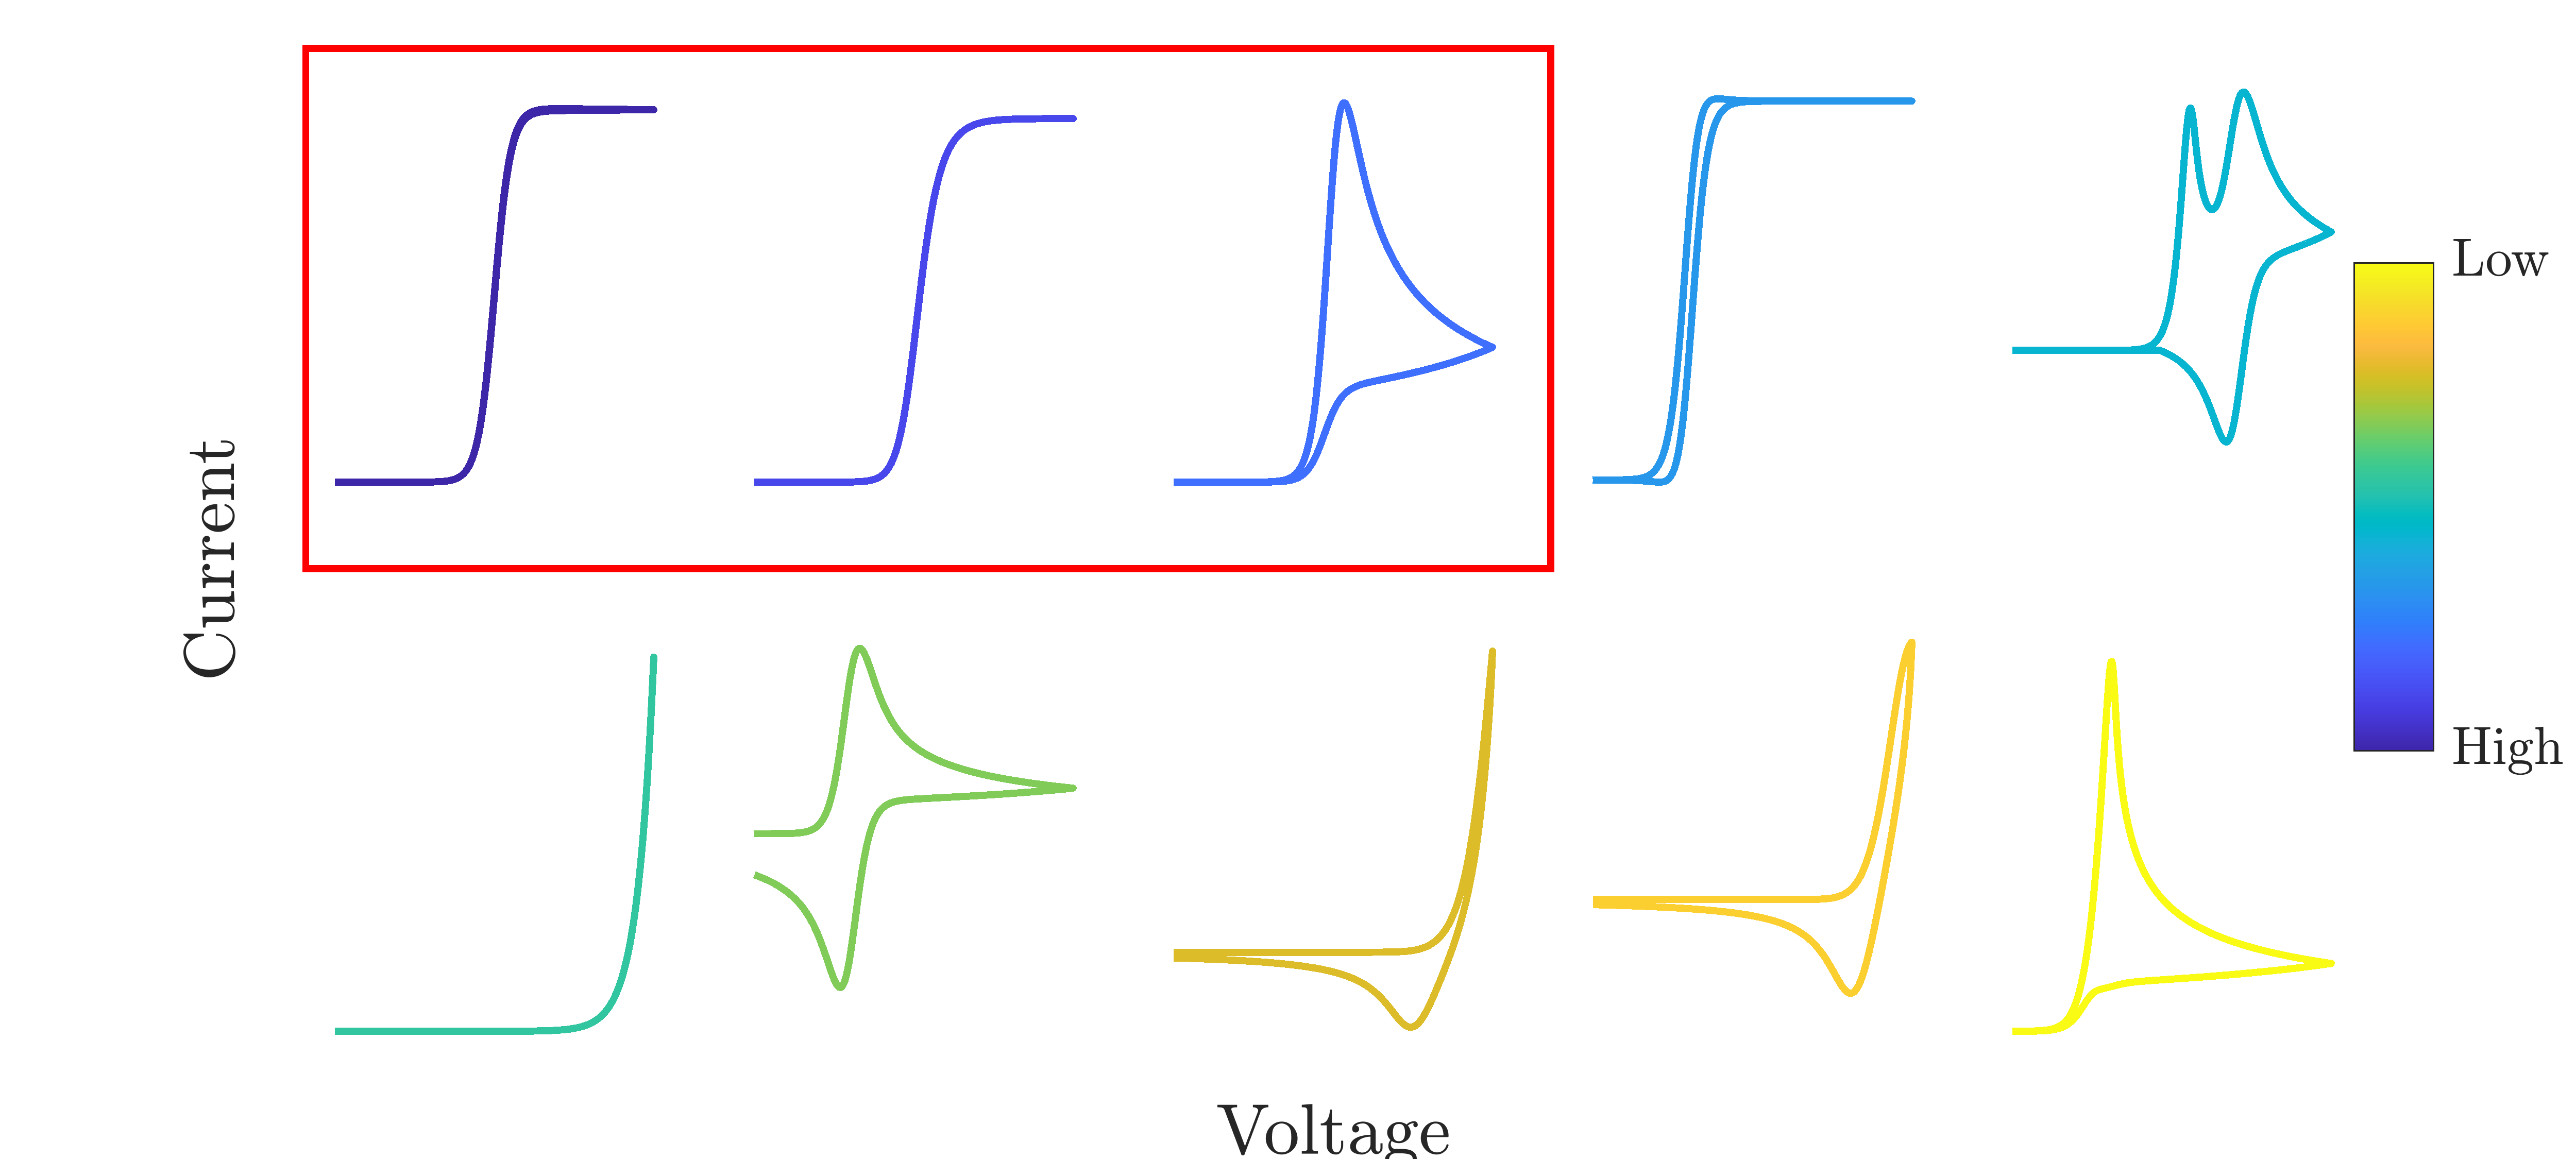
\includegraphics[width=100mm]{Chapter-3/figures/repsimscorespectrum.png}
    \caption{Representative CV curves from the dataset ordered and color coded using the similarity score. CV curves in the red box will be labelled as targets by the similarity score based oracle described here.}
    \label{figSI:repssscores}
\end{figure}

\subsubsection{FOWA-based score} 
In this subsection, a scoring method using the Foot of The Wave Analysis~(FOWA) ~\cite{costentin2015cyclic} is derived.
In the FOWA analysis, the original signal \((I,V)\) is transformed using the map \((I,V)\mapsto(I,1+\exp[\frac{F}{RT}(E-E^0)])\). 
An S-shaped CV curve is expected to be linear in two-dimensional FOWA coordinate space. 
Thus, a CV curve is scored based on its \(R^2\)-value computed with reference to user defined reference S-shape (for multiple S-shaped CV curves, maximum \(R^2\) value over the set is used), quantifying the linearity of the curve after the FOWA transformation.
~\Cref{figSI:repfowascores} is similar to~\Cref{fig:repbmsscores} with the rank of the curves determined by FOWA-based score. 
FOWA-based score ranks two of the target S-shaped CV curves in the top category. 
However, it fails to rank another S-shaped CV curve, like the fourth curve with a current onset only slightly shifted.
When discussing the effectiveness, we note that both of the approaches mentioned in this section depend on the usage of reference S-shapes from which the \(R^2\) value is computed. 
In particular, user needs to select a set of S-shapes that span the expected range in terms of current onset, rate constant etc., which is a non-trivial choice and adds to the heuristics. 
For these reasons BMS is preferred as it exploits the geometrical shape of CV curves directly without need for any user defined references. 
Moreover, note that BMS has an inherent ability to account for Gaussian noise. 
\begin{figure}[h]
    \centering
    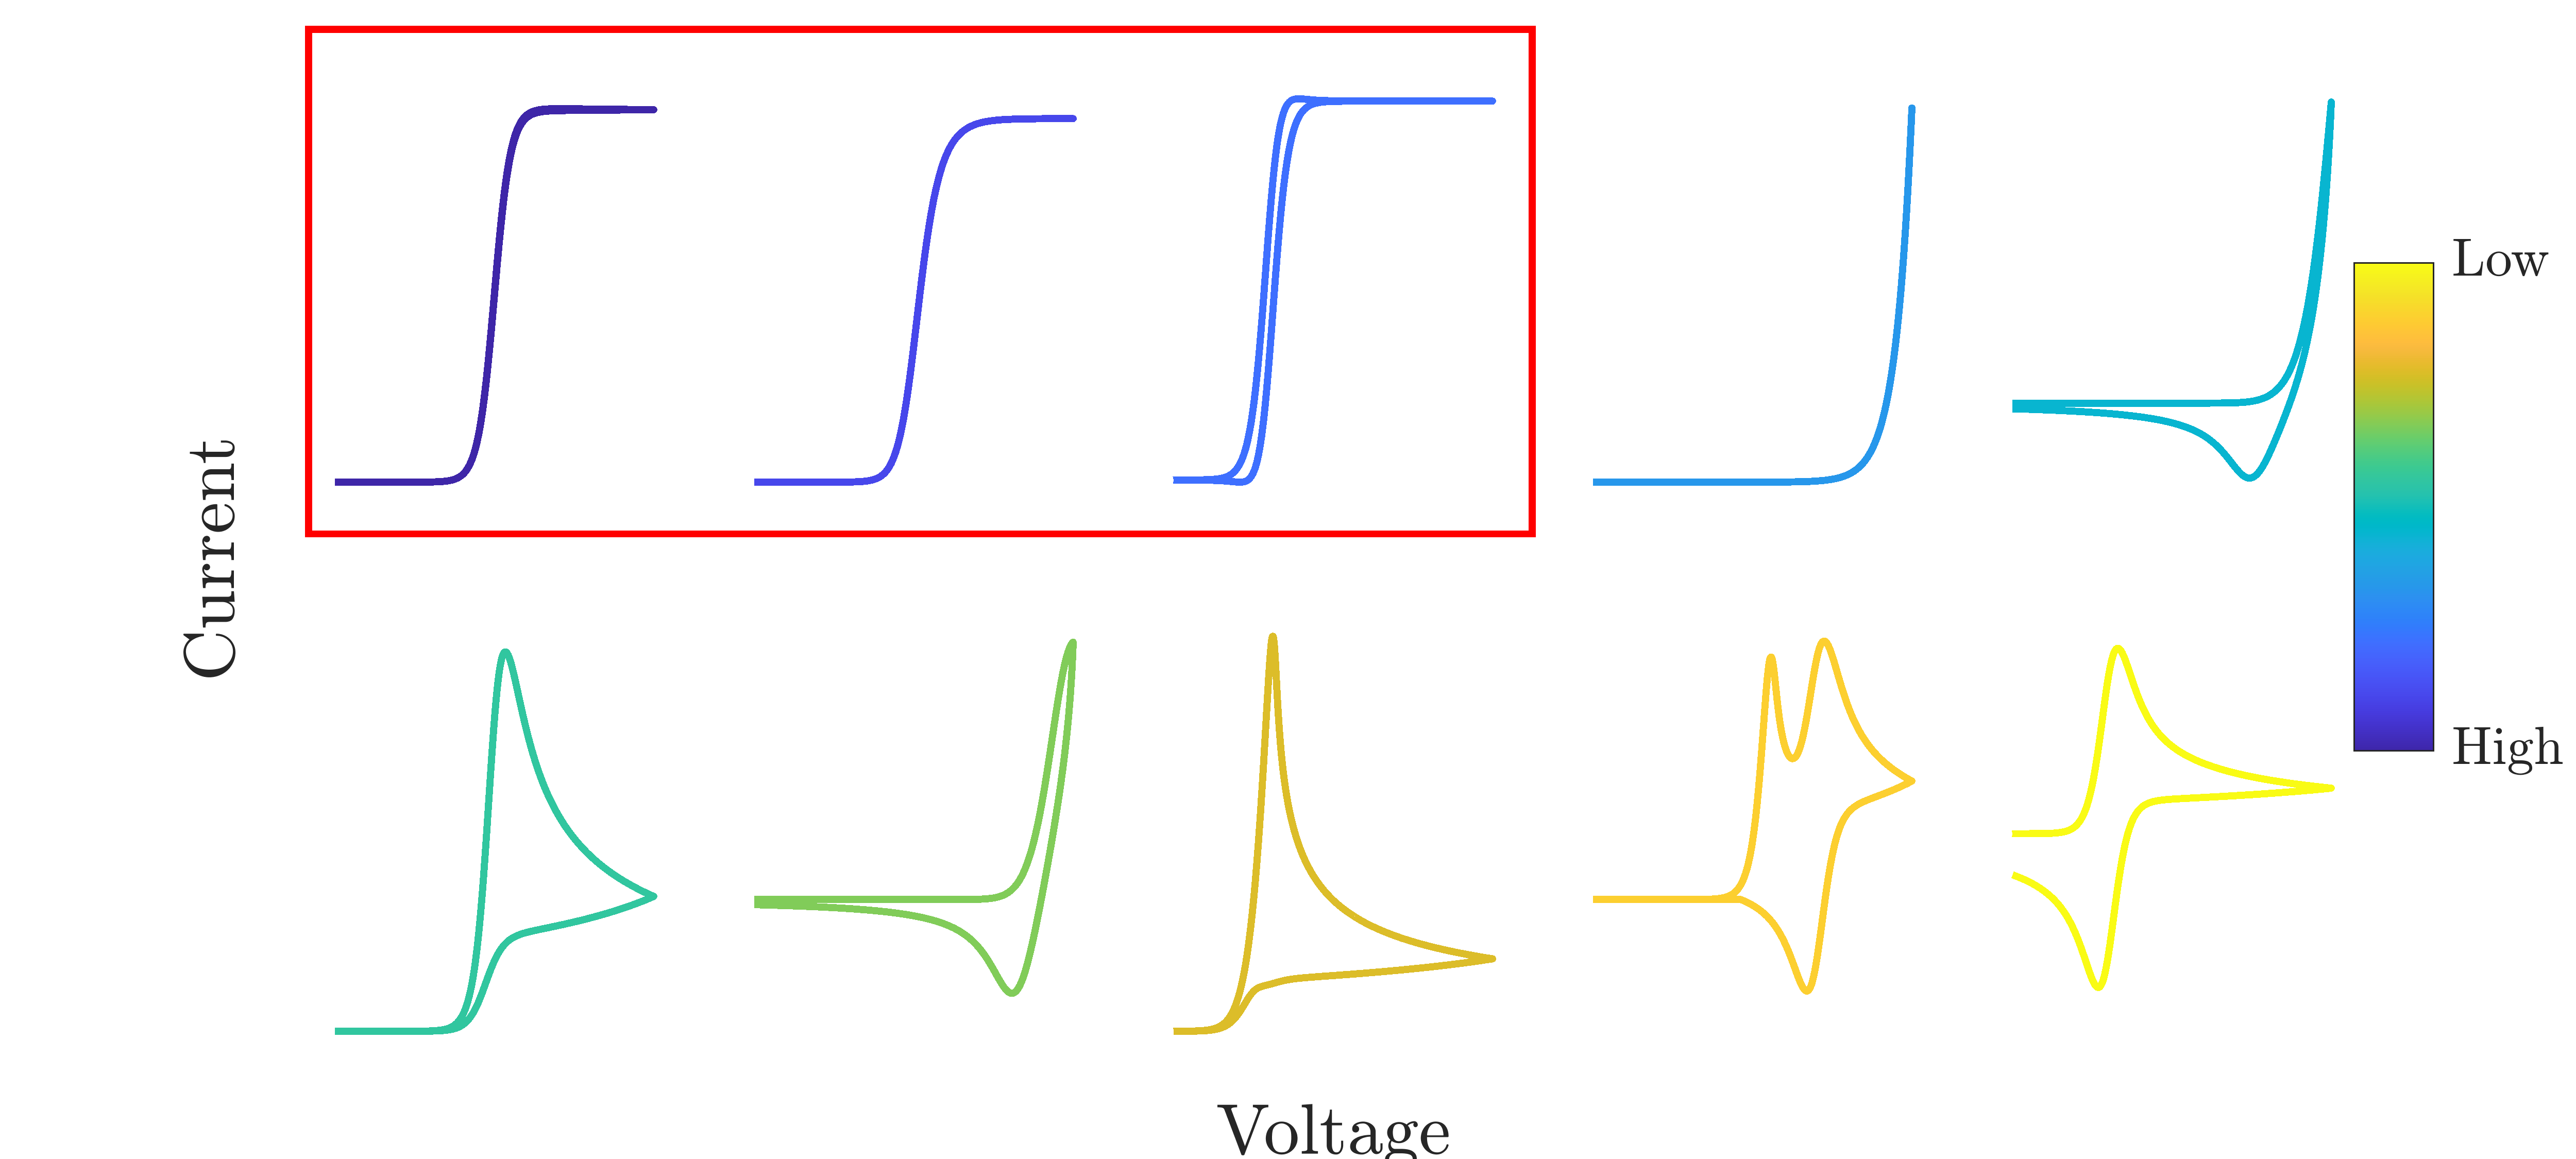
\includegraphics[width=100mm]{Chapter-3/figures/repfowaspectrum.png}
    \caption{Representative CV curves from the dataset ordered and color coded using the FOWA score. CV curves in the red box will be labelled as targets by the similarity FOWA score based oracle described here}
    \label{figSI:repfowascores}
\end{figure}

\section{Active (Batch)Search for S-shaped CV curves}
Active search with batch selection of locations in the design space has been recently studied and successfully applied to  high throughput combinatorial search of material and drug discovery~\cite{jiang2018efficient}. 
We use the state-of-the-art active batch search introduced in Jiang et.al~\cite{jiang2018efficient}, with a fixed budget of 1000 queries~(\(\approx6\%\) of exhaustive search over the grid \(\mathcal{S}\) in \Cref{tab:search_space}) to the simulator for batch sizes of \(b\in\{1,100\}\) to actively query our combinatorial search space~\(\mathcal{S}\).
The batch size reflects the setting of the high throughput analysis, as often material is prepared in batches.

A label for any given location is assigned based on the application of BMS oracle to the corresponding CV curve \(I(v,t)\) simulated by solving~\Cref{{eq:fickslaws,eq:bcs}} over \(4\times10^3\) discrete time points. 
A CV response is labelled as target if its BMS oracle score is in the range defined by top three percentile ranks~\footnote{this is a heuristic and can be altered based on application}~\footnote{Similarly for active search of bi-functional oxygen electrocatalysts, one can assign a material as a target if both of its OER and ORR experimental CV curves are in the top three percentile ranks of BMS scores. } shown in~\Cref{fig:repbmsscores}. 

\begin{figure}[h]
    \centering
    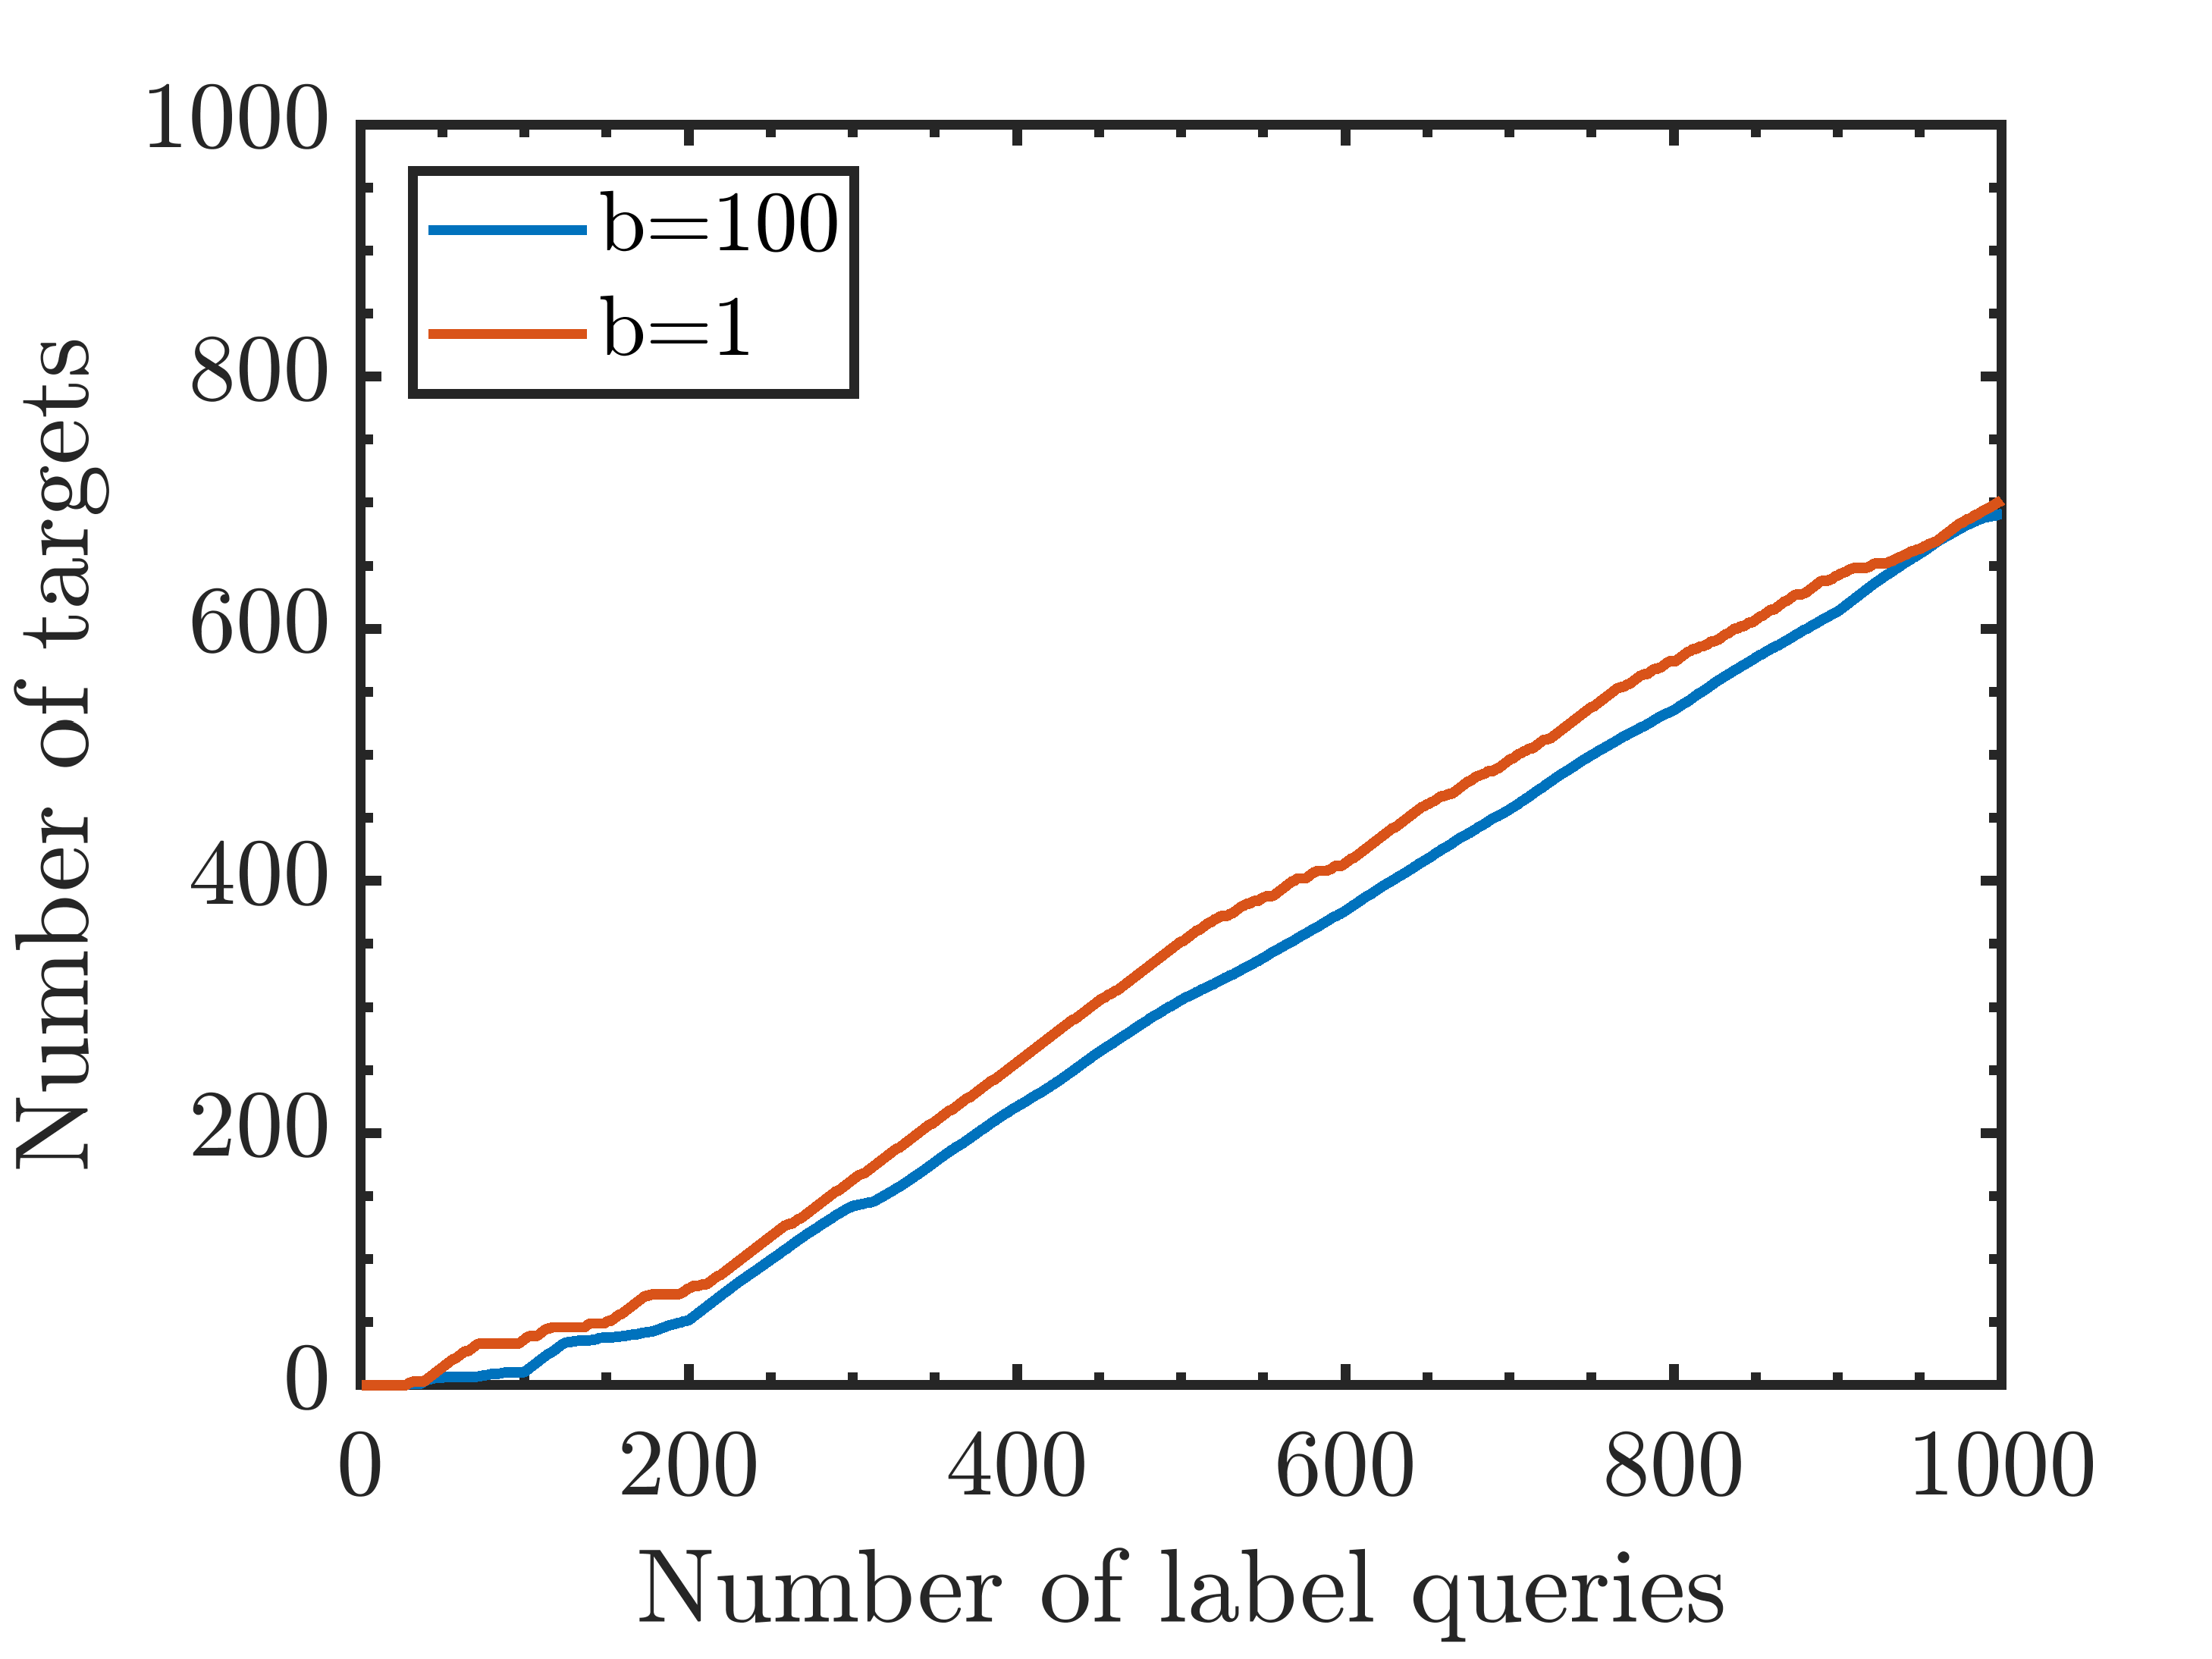
\includegraphics[width=100mm]{Chapter-3/figures/batch_results.png}
    \caption{Active target detection in the EC mechanism combinatorial search space (see~\Cref{tab:search_space} for definition of search space). We repeat the active search 20 times, each time starting with a randomly chosen non-S-shape data point in \(\mathcal{S}\). }
    \label{fig:batchens_fullec}
\end{figure}

Assuming that the design space is continuous, a \(k\)-nearest neighbor probability distribution is used a decision model in Bayesian active learning following the approach in~\cite{jiang2018efficient}. 
This assumption implies that if we find a target at a certain location in the search space, \(k\)-closest neighbors in the design space also are highly likely to be a target as well. 



In~\Cref{fig:batchens_fullec}, we report the average number of targets found in the design space over the number of label queries for two batch sizes \((b=1,100)\) considered~\footnote{The number of targets are averaged over a total of 20 active searches each time start with a randomly selected sample in the search space}.
Our results demonstrate that searching the design space using active learning can be useful, with a near linear target detection. 
It can also be noted from~\Cref{fig:batchens_fullec} for any given number of allowed label queries to the oracle~(or equivalently number of simulation queries to the simulator), the sequential selection finds marginally more targets than the batch selection \(b=100\).
This observation is in accordance with Theorem 1 in~\cite{jiang2018efficient}. 
Jiang et.al,~\cite{jiang2018efficient} argue that batch selection suffers from having to select a batch from the search space with fewer observed responses and locations. 
However, from experimental point of view, one need to consider the advantages and dis-advantages of sequential selection over batch selection. 
